\usepackage{graphicx}
\newpage
\thispagestyle{fancy}
\vspace{\fill}

\subsection{Velocidade da máquina}
\begin{figure}
    \centering
    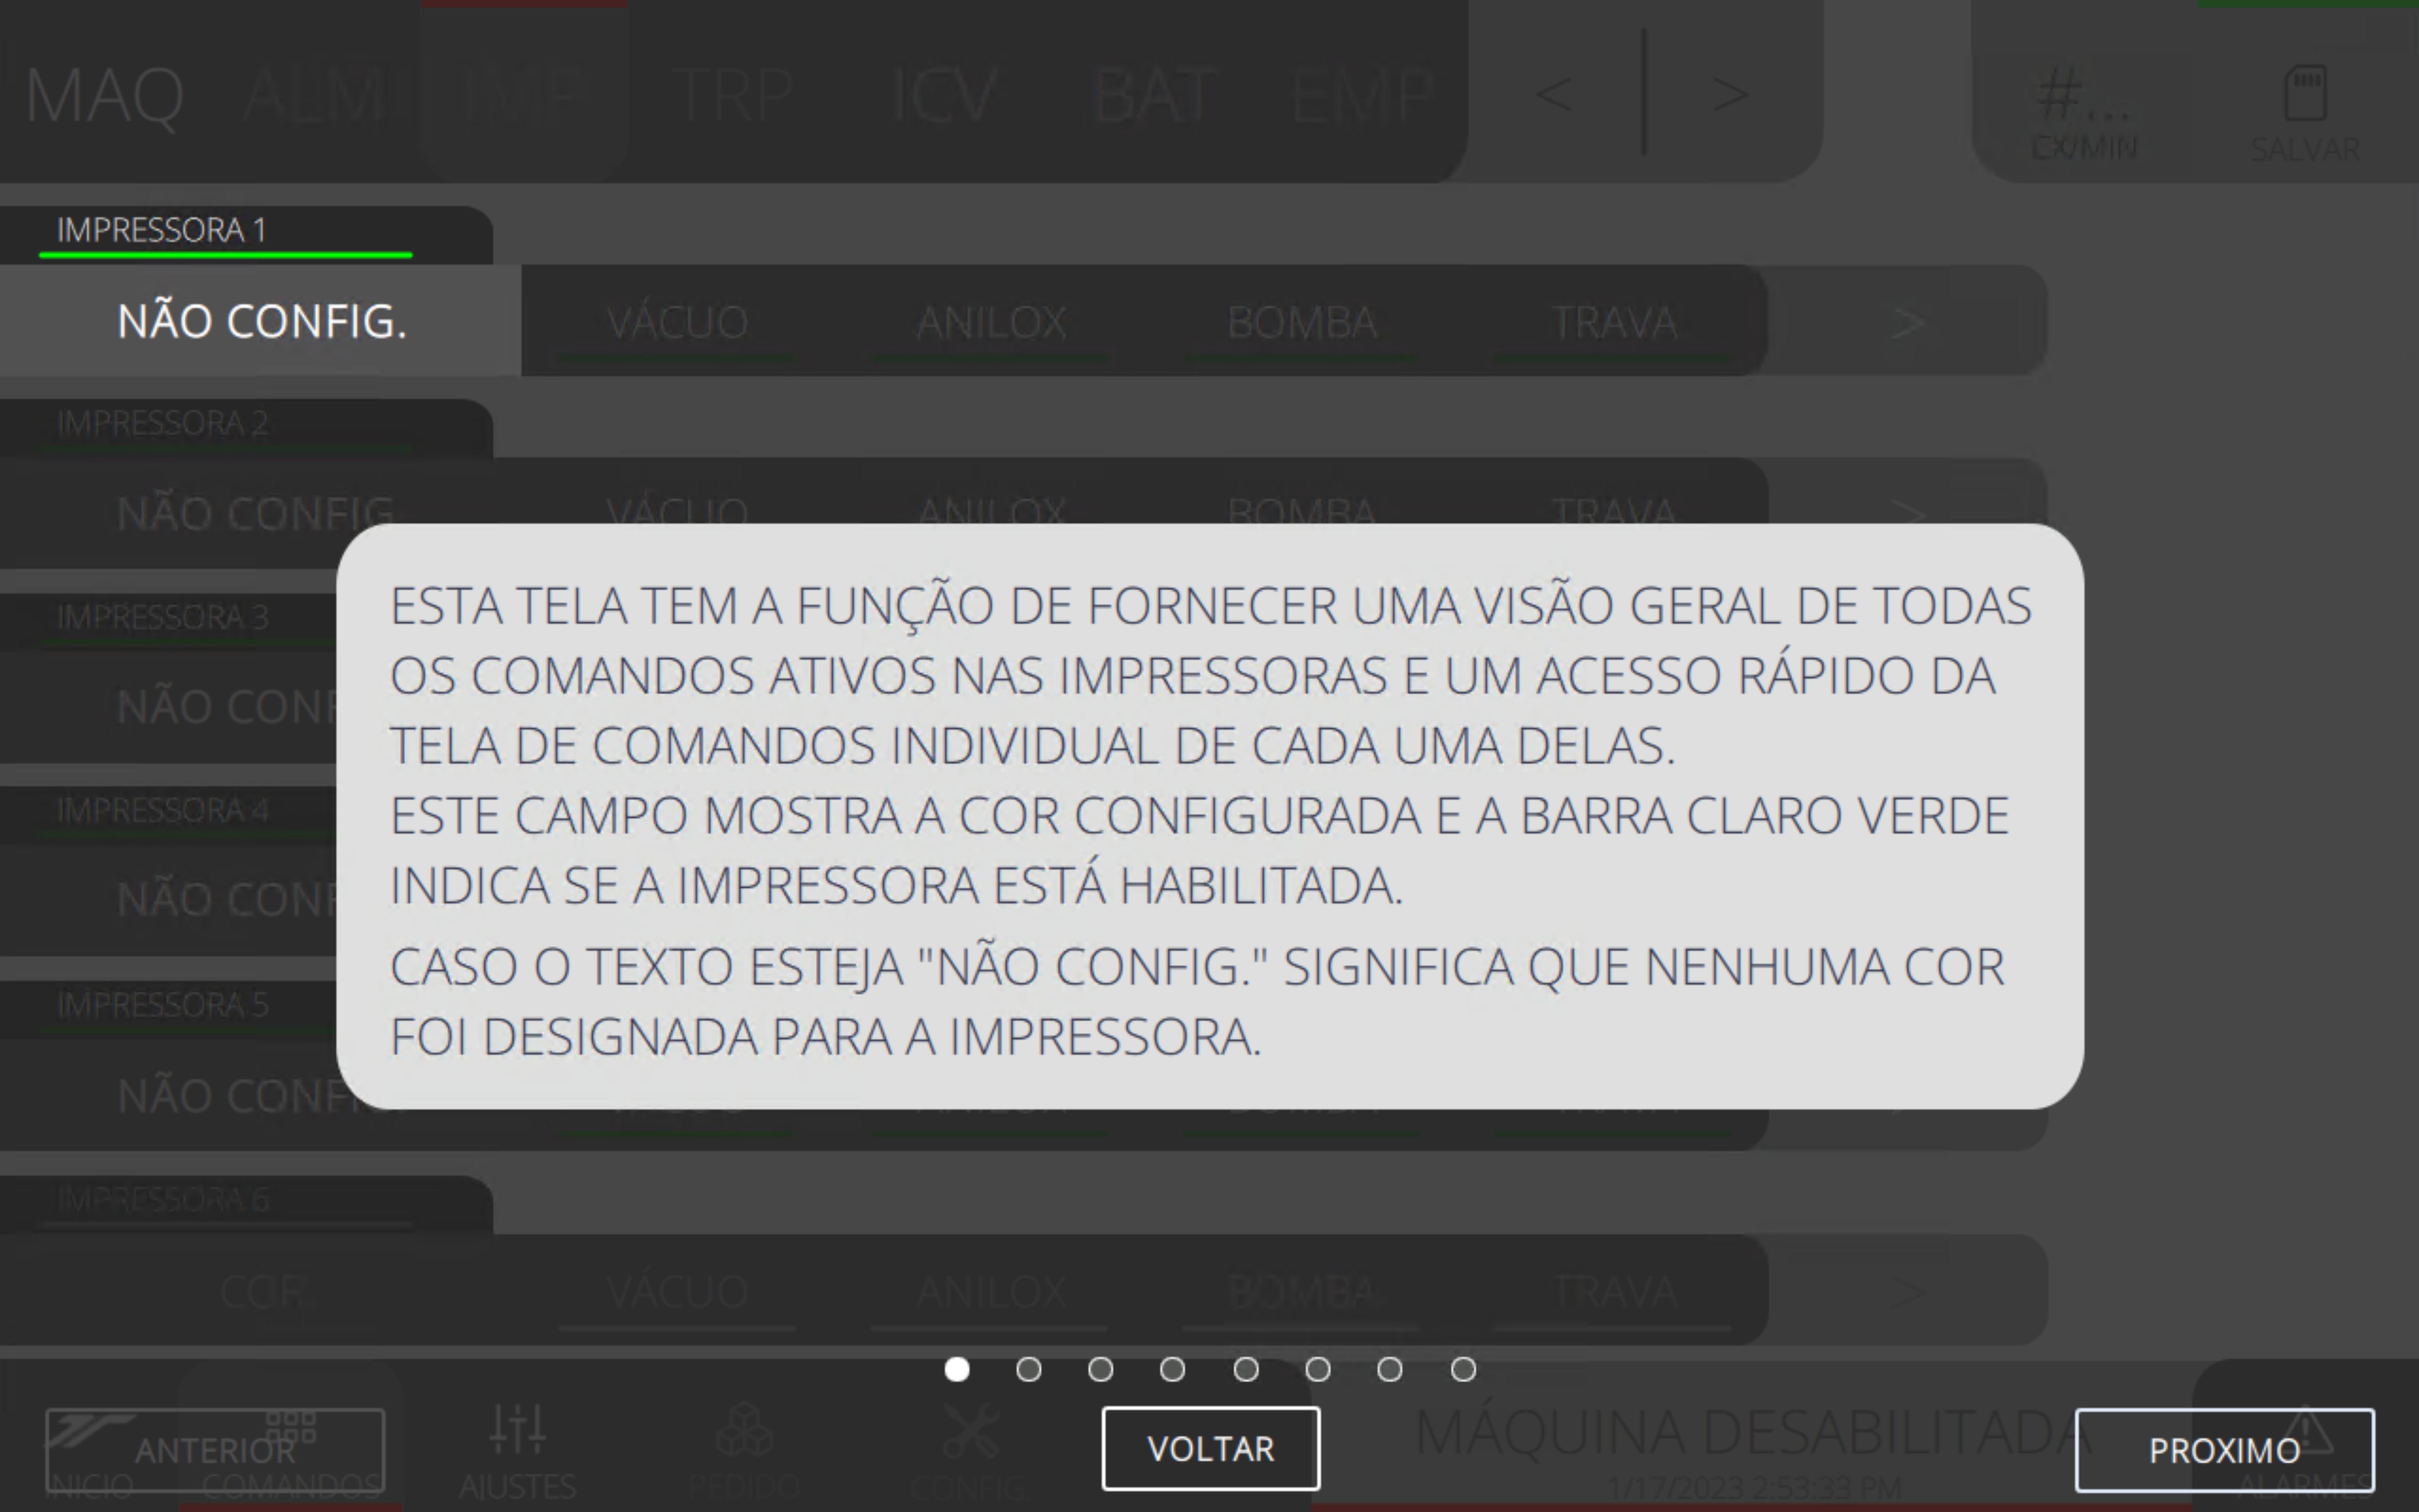
\includegraphics[width=480,height=300]{imagesICV/04-printters/02-printter/commands/1}
    \caption{Velocidade da máquina}
\end{figure}
\newpage
\thispagestyle{fancy}
\vspace{\fill}

\subsection{Executa lavagem de tinta}
\begin{figure}
    \centering
    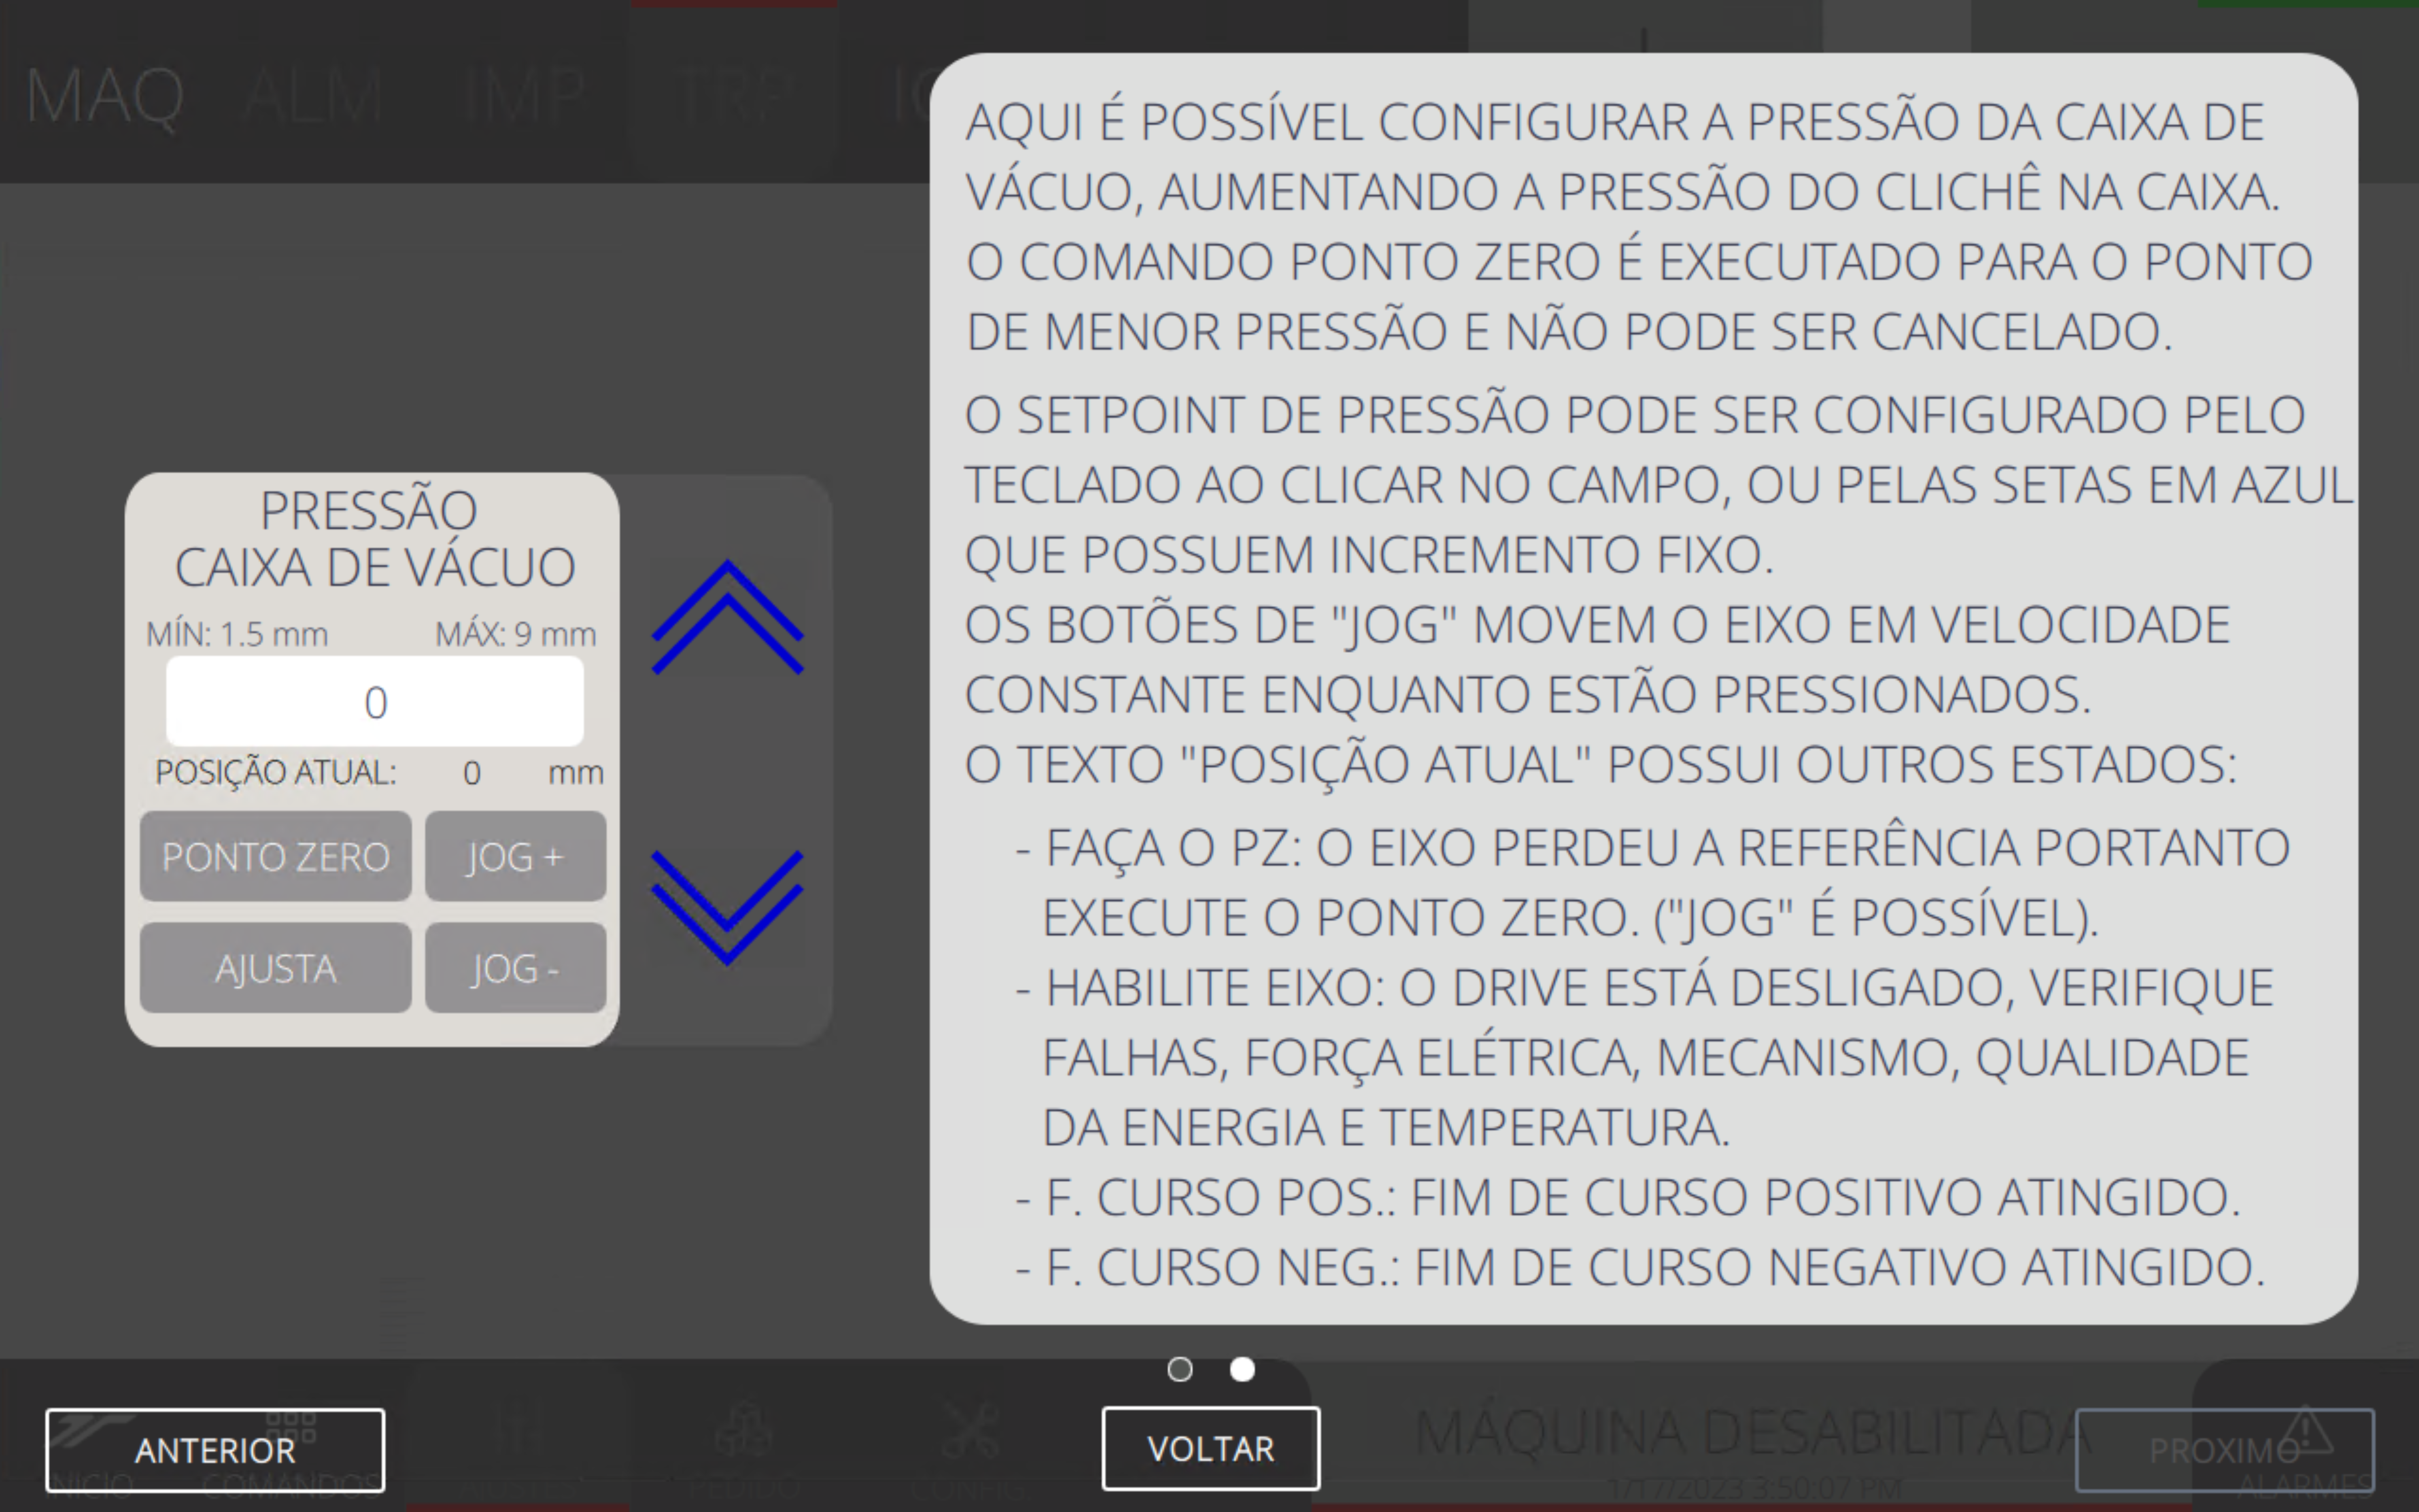
\includegraphics[width=576,height=360]{imagesICV/04-printters/02-printter/commands/2}
    \caption{Executa lavagem de tinta}
\end{figure}
\newpage
\thispagestyle{fancy}
\vspace{\fill}

\subsection{Trava impressora}
\begin{figure}
    \centering
    \includegraphics[width=576,height=360]{imagesICV/04-printters/02-printter/commands/3}
    \caption{\newpage \thispagestyle{fancy} \vspace{\fill}}
\end{figure}
\newpage
\thispagestyle{fancy}
\vspace{\fill}

\subsection{Habilita giro rolo anilox}
\begin{figure}
    \centering
    \includegraphics[width=576,height=360]{imagesICV/04-printters/02-printter/commands/4}
    \caption{Habilita giro rolo anilox}
\end{figure}
\newpage
\thispagestyle{fancy}
\vspace{\fill}

\subsection{Executa ponto zero}
\begin{figure}
    \centering
    \includegraphics[width=576,height=360]{imagesICV/04-printters/02-printter/commands/5}
    \caption{Executa ponto zero}
\end{figure}
\newpage
\thispagestyle{fancy}
\vspace{\fill}

\subsection{Liga bomba de tinta}
\begin{figure}
    \centering
    \includegraphics[width=576,height=360]{imagesICV/04-printters/02-printter/commands/6}
    \caption{Liga bomba de tinta}
\end{figure}
\newpage
\thispagestyle{fancy}
\vspace{\fill}

\subsection{Habilita impressora}
\begin{figure}
    \centering
    \includegraphics[width=576,height=360]{imagesICV/04-printters/02-printter/commands/7}
    \caption{Habilita impressora}
\end{figure}
